\chapter{Conclusion}
brief of conclusion
\maxdeadcycles=200
\extrafloats{100}

\section{Cokro Edi Prawiro / 1164069}

\subsection{Teori}
\begin{enumerate}

\item Jelaskan Kenapa Kata-Kata harus dilakukan vektorisasi lengkapi dengan ilustrasi gambar.\par
Kata kata harus dilakukan vektorisasi dikarenakan atau bertujuan utk mengukur nilai kemunculan suatau kata yang serupa dari sebuah kalimat sehingga kata-kata tersebut dapat di prediksi kemunculanya. atau juga di buatnya vektorisasi data digunakan untuk memprediksi bobot dari suatu kata misalkan ayam dan kucing sama-sama hewan maka akan dibuat prediksi apakah kata tersebut akan muncul pada kalimat yang kira-kira memiliki bobot yang sama. untuk dapat jelasnya dapat melihat ilustrasi pada gambar \ref{c71}.

\begin{figure}[!htbp]
      \centering{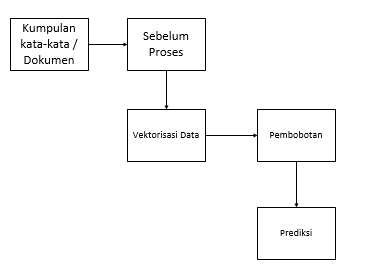
\includegraphics[width=0.5\textwidth]
      {figures/cokro/c71}}
      \caption{Ilustrasi Vektorisasi Kata-Kata}
      \label{c71}
      \end{figure}

\item Jelaskan Mengapa dimensi dari vektor dataset google bisa mencapai 300 lengakapi dengan ilustrasi gambar. \par
Dimensi dataset dari google bisa mencapai 300 karena dimensi dari vektor tersebut digunakan untuk membandingkan bobot dari setiap kata, misalkan terdapat kata dog dan cat pada dataset google tersebut setiap kata tersebut di buat dimensi vektor 300 untuk kata dog dan 300 dimensi vektor juga untuk kata cat kemudian kata tersebt di bandingkan bobot kesamaan katanya maka akan muncul akurasi sekitar 70 persen kesamaan bobot dikarenakan kata dog dan cat sama sama di gunakan untuk hewan priharaan. untuk lebih jelasnya dapat dilihat pada gambar \ref{c72}.

\begin{figure}[!htbp]
      \centering{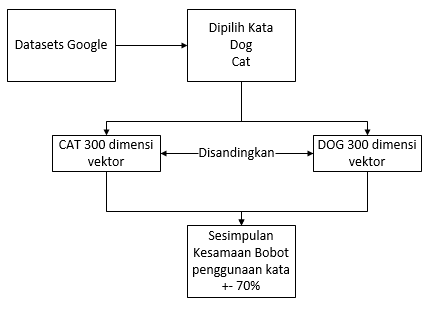
\includegraphics[width=0.5\textwidth]
      {figures/cokro/c72}}
      \caption{Ilustrasi Kenapa dimensi vektor pada datasets google haris 300}
      \label{c72}
      \end{figure}

\item Jelaskan Konsep vektorisasi untuk kata . dilengkapi dengan ilustrasi atau gambar. \par
Vektorisasi untuk kata untuk mengetahui kata tengah dari suatau kalimat atau kata utama atau objek utama pada suatau kalimat contoh ( Jangan lupa subscribe channel saya ya sekian treimakasih ) kata tengah tersebut merupakan channel yang memiliki bobot sebagai kata tengah dari suatu kalimat atau bobot sebagai objek dari suatu kalimat. hal ini sangat berkaitan dengan dimensi vektor pada dataset google yang 300 tadi karena untuk mendapatkan nilai atau bobot dari kata tengah tersebut di dapatkan dari proses dimensiasi dari kata tersebut. untuk lebih jelasnya dapat dilihat pada gambar \ref{c73} berikut :

\begin{figure}[!htbp]
      \centering{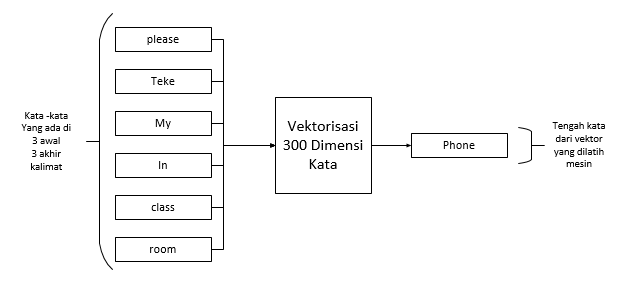
\includegraphics[width=0.5\textwidth]
      {figures/cokro/c73}}
      \caption{Ilustrasi konsep vektorisasi untuk kata}
      \label{c73}
      \end{figure}

\item Jelaskan Konsep vektorisasi untuk dokumen. dilengkapi dengan ilustrasi atau gambar. \par
Vektorisasi untuk dokumen hampir sama seperti vektorisasi untuk kata hanya saja pemilihan kata utama atau kata tengah terdapat pada satu dokumen jadi mesin akan membuat dimensi vektor 300 untuk dokumen dan nanti kata tengahnya akan di sandingkan pada dokumen yany terdapat pada dokumen tersebut contoh dapat dilihat pada gambar \ref{c74} berikut : 

\begin{figure}[!htbp]
      \centering{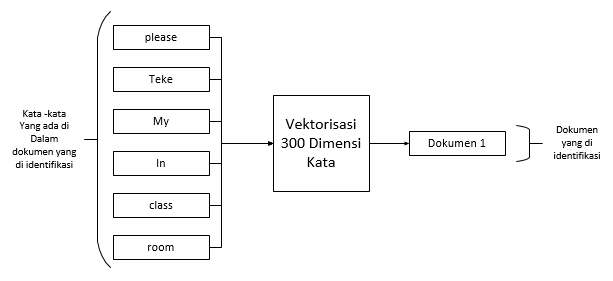
\includegraphics[width=0.5\textwidth]
      {figures/cokro/c74}}
      \caption{Ilustrasi konsep vektorisasi untuk dokumen}
      \label{c74}
      \end{figure}

\item Jelaskan apa mean dan standar deviasi, lengkapi dengan iludtrasi atau gambar. \par
mean merupakan petunjuk terhadap kata-kata yang di olah jika kata kata itu akurasinya tinggi berarti kata tersebut sering muncul begitu juga sebaliknya untuk lebih jelasnya dapat dilihat pada gambar \ref{c75} sedangkan setandar defiation merupakan standar untuk menimbang kesalahan. sehingga kesalahan tersebut di anggap wajar misarkan kita memperkirakan kedalaman dari dataset merupakan 2 atau 3 tapi pada kenyataanya merupakan 5 itu merupakan kesalahan tapi masih bisa dianggap wajar karna masih mendekati perkiraan awal.

\begin{figure}[!htbp]
      \centering{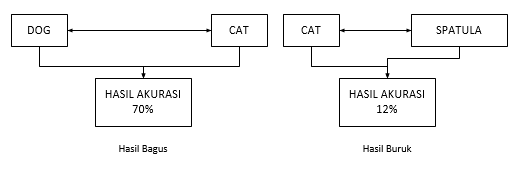
\includegraphics[width=0.5\textwidth]
      {figures/cokro/c75}}
      \caption{Ilustrasi Penggunaan Mean}
      \label{c75}
      \end{figure}

\item Jelaskan Apa itu Skip-Gram sertakan contoh ilustrasi. \par
Skip-Gram adalah kebalikan dari konsep vektorisasi untuk kata dimana kata tengah menjadi acuan terhadap kata kata pelengkap dalam suatu kalimat untuk lebih jelasnya dapat di lihat pada gambar \ref{c76} berikut :

\begin{figure}[!htbp]
      \centering{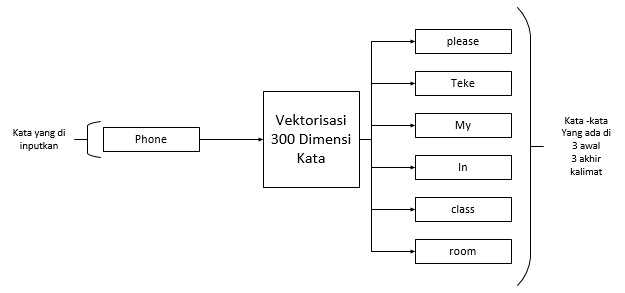
\includegraphics[width=0.5\textwidth]
      {figures/cokro/c76}}
      \caption{Ilustrasi Skip-Gram}
      \label{c76}
      \end{figure}

\end{enumerate}
\subsection{Praktikum}
\begin{enumerate}
\item mencoba dataset google dan penjelasan vektor dari kata love, faith, fall, sick, clear, shine, bag, car, wash, motor, dan cycle.\par

\begin{itemize}
\item berikut merupakan code import gensim digunakan untuk membuat data model atau rangcangan data yang akan di buat. selanjutnya dibuat variabel gmodel yang berisi data vektor negativ. selanjutnya data tersebut di load agar data tersebut dapat di tampilkan dan di olah. code lengkapnya dapat dilihat pada gambar \ref{c89}.

\begin{figure}[!htbp]
      \centering{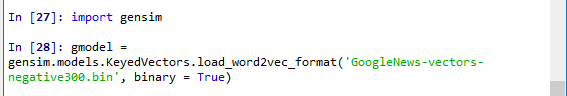
\includegraphics[width=0.5\textwidth]
      {figures/cokro/c89}}
      \caption{Import Gensim dan membuat model gmodel}
      \label{c89}
      \end{figure}

\item berikut merupakan hasil lpengolahan kata clear pada data google yang di load tadi. Sehingga memunculkan hasil vektor 300 dimensi untuk kata tersebut. untuk jelasnya dapat di lihat pada gambar \ref{c77}.
\begin{figure}[!htbp]
      \centering{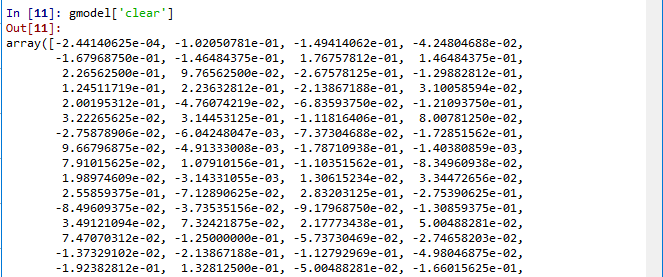
\includegraphics[width=0.5\textwidth]
      {figures/cokro/c77}}
      \caption{Hasil Matrix Clear}
      \label{c77}
      \end{figure}

\item berikut merupakan hasil lpengolahan kata Shine pada data google yang di load. Sehingga memunculkan hasil vektor 300 dimensi untuk kata tersebut. untuk jelasnya dapat di lihat pada gambar \ref{c78}.

\begin{figure}[!htbp]
      \centering{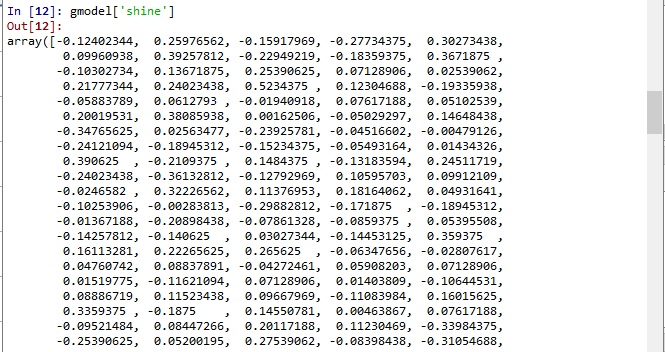
\includegraphics[width=0.5\textwidth]
      {figures/cokro/c78}}
      \caption{Hasil Matrix Shine}
      \label{c78}
      \end{figure}

\item berikut merupakan hasil lpengolahan kata bag pada data google yang di load. Sehingga memunculkan hasil vektor 300 dimensi untuk kata tersebut. untuk jelasnya dapat di lihat pada gambar \ref{c79}.

\begin{figure}[!htbp]
      \centering{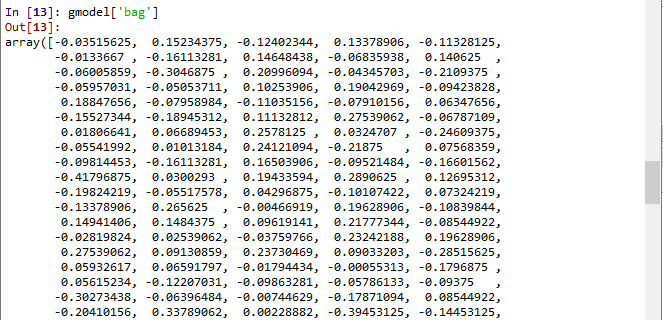
\includegraphics[width=0.5\textwidth]
      {figures/cokro/c79}}
      \caption{Hasil Matrix bag}
      \label{c79}
      \end{figure}

\item berikut merupakan hasil lpengolahan kata Car pada data google yang di load. Sehingga memunculkan hasil vektor 300 dimensi untuk kata tersebut. untuk jelasnya dapat di lihat pada gambar \ref{c80}.

\begin{figure}[!htbp]
      \centering{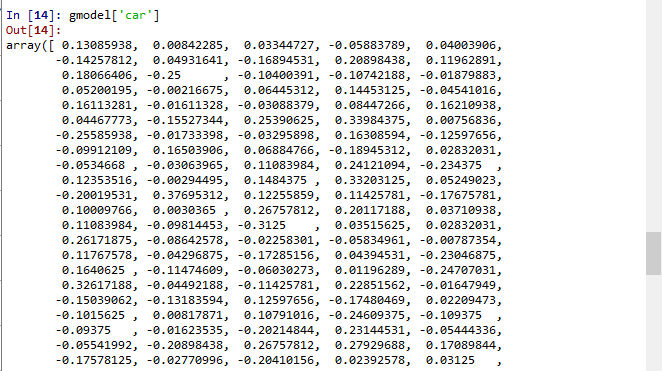
\includegraphics[width=0.5\textwidth]
      {figures/cokro/c80}}
      \caption{Hasil Matrix Car}
      \label{c80}
      \end{figure}


\item berikut merupakan hasil lpengolahan kata Wash pada data google yang di load. Sehingga memunculkan hasil vektor 300 dimensi untuk kata tersebut. untuk jelasnya dapat di lihat pada gambar \ref{c81}.

\begin{figure}[!htbp]
      \centering{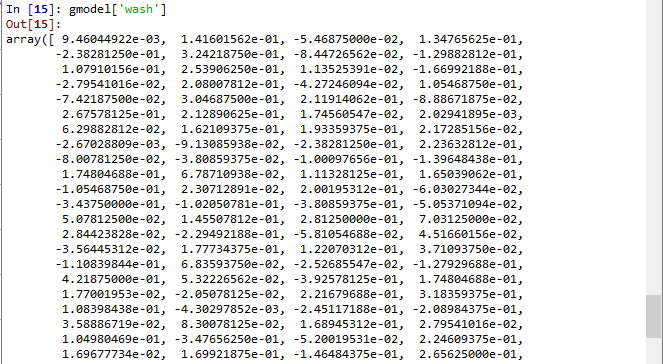
\includegraphics[width=0.5\textwidth]
      {figures/cokro/c81}}
      \caption{Hasil Matrix Wash}
      \label{c81}
      \end{figure}

\item berikut merupakan hasil lpengolahan kata Motor pada data google yang di load. Sehingga memunculkan hasil vektor 300 dimensi untuk kata tersebut. untuk jelasnya dapat di lihat pada gambar \ref{c82}.

\begin{figure}[!htbp]
      \centering{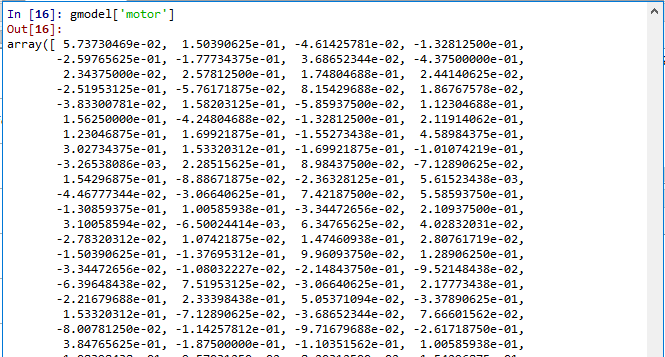
\includegraphics[width=0.5\textwidth]
      {figures/cokro/c82}}
      \caption{Hasil Matrix Motor}
      \label{c82}
      \end{figure}

\item berikut merupakan hasil lpengolahan kata Cycle pada data google yang di load. Sehingga memunculkan hasil vektor 300 dimensi untuk kata tersebut. untuk jelasnya dapat di lihat pada gambar \ref{c83}.

\begin{figure}[!htbp]
      \centering{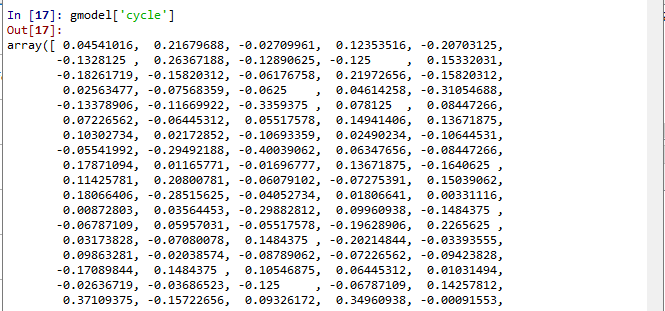
\includegraphics[width=0.5\textwidth]
      {figures/cokro/c83}}
      \caption{Hasil Matrix Cycle}
      \label{c83}
      \end{figure}

\item berikut merupakan hasil lpengolahan kata love pada data google yang di load. Sehingga memunculkan hasil vektor 300 dimensi untuk kata tersebut. untuk jelasnya dapat di lihat pada gambar \ref{c84}.

\begin{figure}[!htbp]
      \centering{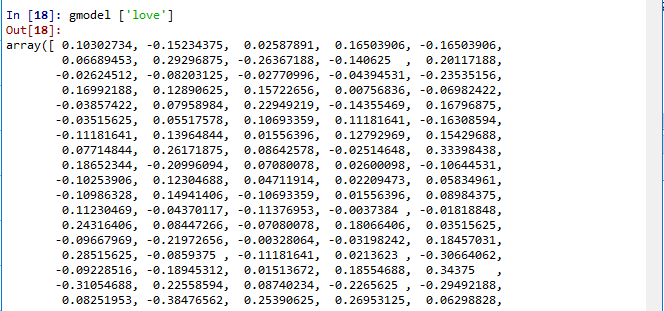
\includegraphics[width=0.5\textwidth]
      {figures/cokro/c84}}
      \caption{Hasil Matrix love}
      \label{c84}
      \end{figure}

\item berikut merupakan hasil lpengolahan kata faith pada data google yang di load. Sehingga memunculkan hasil vektor 300 dimensi untuk kata tersebut. untuk jelasnya dapat di lihat pada gambar \ref{c85}.

\begin{figure}[!htbp]
      \centering{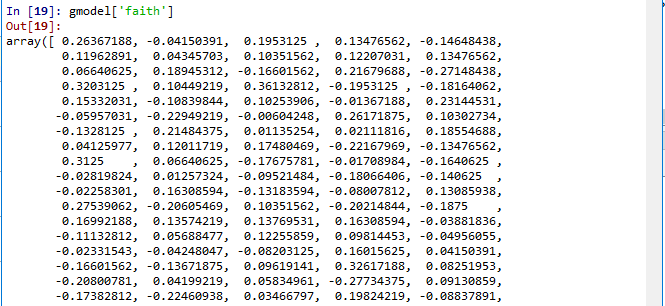
\includegraphics[width=0.5\textwidth]
      {figures/cokro/c85}}
      \caption{Hasil Matrix faith}
      \label{c85}
      \end{figure}

\item berikut merupakan hasil lpengolahan kata Fall pada data google yang di load. Sehingga memunculkan hasil vektor 300 dimensi untuk kata tersebut. untuk jelasnya dapat di lihat pada gambar \ref{c86}.

\begin{figure}[!htbp]
      \centering{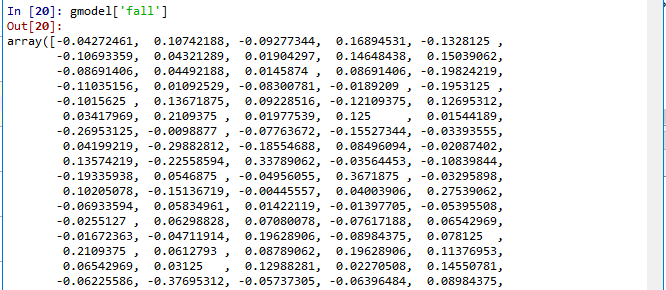
\includegraphics[width=0.5\textwidth]
      {figures/cokro/c86}}
      \caption{Hasil Matrix Fall}
      \label{c86}
      \end{figure}

\item berikut merupakan hasil lpengolahan kata Sick pada data google yang di load. Sehingga memunculkan hasil vektor 300 dimensi untuk kata tersebut. untuk jelasnya dapat di lihat pada gambar \ref{c87}.

\begin{figure}[!htbp]
      \centering{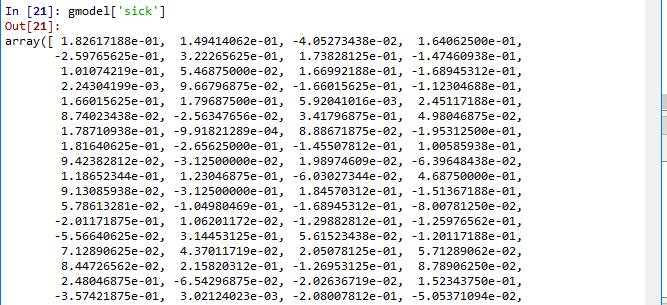
\includegraphics[width=0.5\textwidth]
      {figures/cokro/c87}}
      \caption{Hasil Matrix Sick}
      \label{c87}
      \end{figure}

\item berikut merupakan hasil dari similaritas kata kata yang di olah menjadi matrix tadi adapun persentase untuk perbandingan setiap katanya yaitu 9 persen untuk kata wash dan clear 7 persen untuk kata bag dan love 48 persen untuk kata motor dan car 12 persen untuk kata sick dan faith dan terakhir yaitu 6 persen untuk kata cycle dan shine. untuk jelasnya dapat di lihat pada gambar \ref{c88}.

\begin{figure}[!htbp]
      \centering{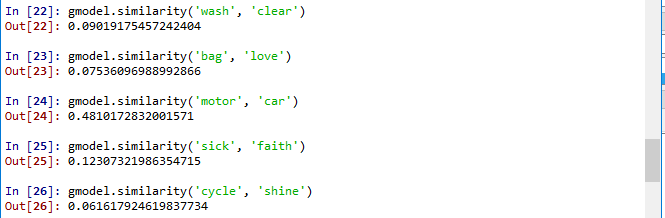
\includegraphics[width=0.5\textwidth]
      {figures/cokro/c88}}
      \caption{hasil dari lima similaritas}
      \label{c88}
      \end{figure}

\end{itemize}

\item pada code berikut merupakan hasil dari running code untu ekstrak word dimana pada baris ke tiga dimasukan perintah untuk menghapus tag html yang terdapat dalam file tesebut selanjutnya pada baris ke 4 yaitu perintah untuk menghilangkan tanda kutip satu selanjutnya pada baris ke 5 yaitu perintah untuk menghapus tanda baca pada file tersebut dan yang terakhir yaitu perintah untuk menghapus dable sepasi atau sepasi berurutan. setelah itu dibuat clas bari dari random yang bertujuan untuk mengkocok data yang ada pada file tersebut kemudian class permute sentence tersebut akan di gunkan untuk mengolah data selanjutnya. untuk lebih jelasnya dapat dilihat pada gambar \ref{c90}.

\begin{figure}[!htbp]
      \centering{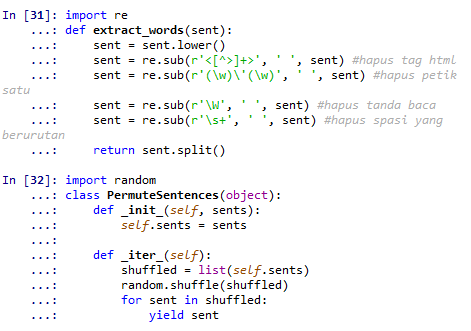
\includegraphics[width=0.5\textwidth]
      {figures/cokro/c90}}
      \caption{hasil dari ekstrak\_words dan permute Sentence}
      \label{c90}
      \end{figure}

\item gensim merupakan library untuk memodelkan topik unsuperpise atau memodelkan bahasa dengan model unsuperpise. Sadangkan taget dokumen digunakan untuk TaggetDokumen berarti memasukan dokumen untuk di olah oleh mesin. Kemudian Doc2Vect dugunakan untuk membandingkan dokumen apakah isi dari dokumen itu bobotnya sama dengan dokumen yang di sandingkannya. untuk lebih jelasnya dapat dilihat pada gambar \ref{c91} pada gambar tersebut menunjukan di baris ke satau dilakukan dari librari gensim dokumen mengimport method taggedDocument lalu pada baris kedua dari librari gensim model melakukan import metod Doc2Vec.

\begin{figure}[!htbp]
      \centering{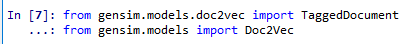
\includegraphics[width=0.5\textwidth]
      {figures/cokro/c91}}
      \caption{Hasil dari penggunaan library gensim , TaggetDocument dan Doc2Vec}
      \label{c91}
      \end{figure}

\item cara memasukan data traning file pertama tentukan terlebih dahulu tempat file dokumen tersebut disimpan kemudian import librari os setelah itu buat variabel unsup\_sentences yang berisikan array kosong, lalu tentukan file yang akan dimasukan setelah itu lakukan os listdir pada data yang akan dimasukan kemudian semua data tersebut di inisialisasi menjadi f kemudian nama f tersebut dimasukan ke variabel unsup untuk lebih jelasnya dapat di lihat pada gambar \ref{c92} berikut. pada codingan tersebut merupakan praktikum untuk memasukan data doc2vec\par

\begin{figure}[!htbp]
      \centering{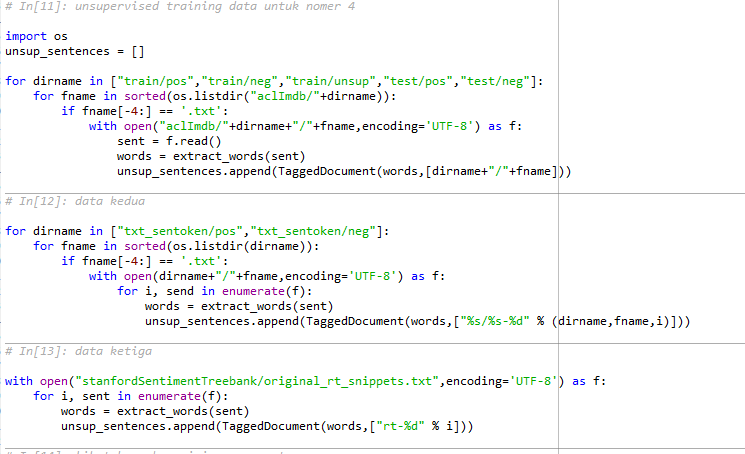
\includegraphics[width=0.7\textwidth]
      {figures/cokro/c92}}
      \caption{Codingan untuk memasukan dokumen pelatihan doc2vec}
      \label{c92}
      \end{figure}

dan untuk hasilruningnya dapat dilihat pada gambar \ref{c93} kemudian hasilnya dapat dilihat pada gambar \ref{c94}  dimana akan muncul dirname, fname, sent, unsup\_sentences dan word dimana data unsup tersebut yang akan di olah nanti sebagai data seting dan terdapat 391 kata dalam file tersebut. setelah itu dilakukan running lagi pada code berikutnya sehingga akan muncul hasil seperti gambar \ref{c95} yang mana coding tersebut berguna untuk menambah data unsup\_sentences menjadi 160 sekian ribu seperti pada gambar \ref{c96}.  Selanjutnya dirunning code ke tiga yang dapat di lihat pada gambar \ref{c97} untuk  menambahkan data menjadi 175 sekian yang hasil akhirnya dapat di lihat pada gambar \ref{c98}  berikut.\par

\begin{figure}[!htbp]
      \centering{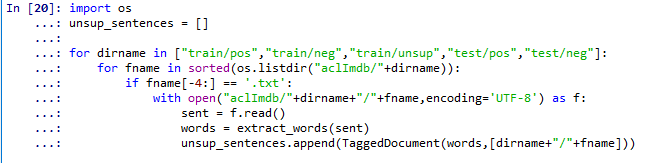
\includegraphics[width=0.7\textwidth]
      {figures/cokro/c93}}
      \caption{hasil running codingan ke 1}
      \label{c93}
      \end{figure}

\begin{figure}[!htbp]
      \centering{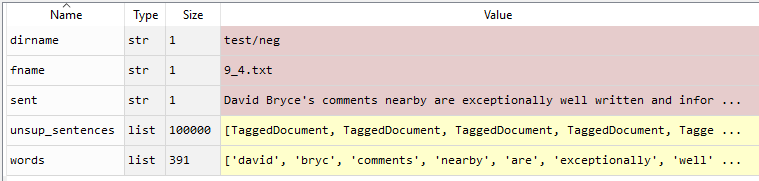
\includegraphics[width=0.7\textwidth]
      {figures/cokro/c94}}
      \caption{Hasil insert data doc2vec dari codingan pertama}
      \label{c94}
      \end{figure}

\begin{figure}[!htbp]
      \centering{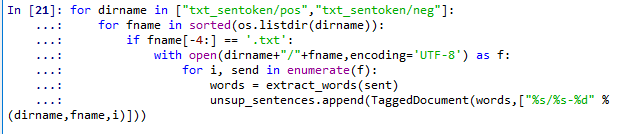
\includegraphics[width=0.7\textwidth]
      {figures/cokro/c95}}
      \caption{hasil running codingan ke 2}
      \label{c95}
      \end{figure}

\begin{figure}[!htbp]
      \centering{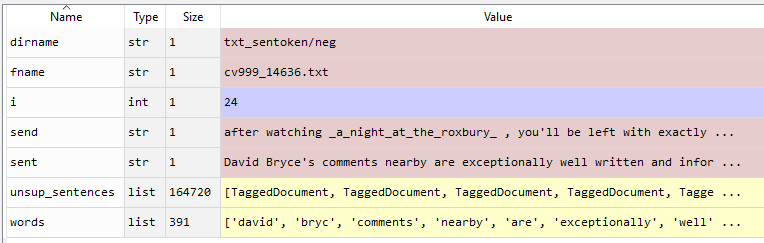
\includegraphics[width=0.7\textwidth]
      {figures/cokro/c96}}
      \caption{Hasil insert data doc2vec dari codingan ke dua}
      \label{c96}
      \end{figure}

\begin{figure}[!htbp]
      \centering{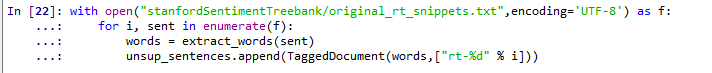
\includegraphics[width=0.7\textwidth]
      {figures/cokro/c97}}
      \caption{hasil running codingan ke 3}
      \label{c97}
      \end{figure}

\begin{figure}[!htbp]
      \centering{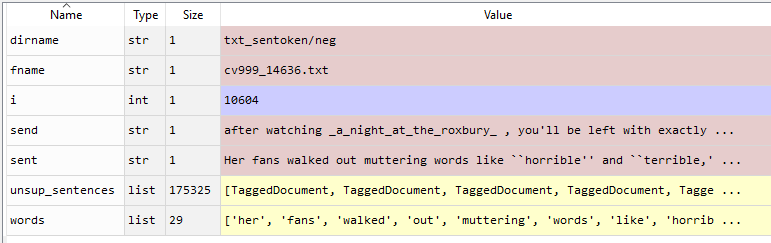
\includegraphics[width=0.7\textwidth]
      {figures/cokro/c98}}
      \caption{Hasil insert data doc2vec dari codingan ke tiga}
      \label{c98}
      \end{figure}

\item kenapa harus dilakukan pengocokan data atau rendomisasi ? hal ini harus dilakukan supaya data lebis gambang untuk di olah dan meningkatkan tingkat akurasi dari proses pengolahan data Doc2Vec. kemudian harus dilakukan pembersihan data agar memori pc atau laptop yang di gunakan untuk mengolah data menjadi ringan dan menambah peforma dari mesin itu sendiri untuk codingan pertama lakukan terlebih dahulu rendomisasi. dapat di lihat pada gambar \ref{c99} selanjutnya membuat variabel baru dengan nama mute yang di isi data class random dan data unsup\_sentence yang dapat dilihat pada gambar \ref{c100}. kemudian setelah pengolahan data dilakukan pembersihan dengan melakukan code pada gambar \ref{c101}

\begin{figure}[!htbp]
      \centering{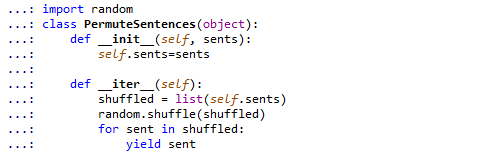
\includegraphics[width=0.7\textwidth]
      {figures/cokro/c99}}
      \caption{Membuat random dan membuat class PermuteSentence}
      \label{c99}
      \end{figure}

\begin{figure}[!htbp]
      \centering{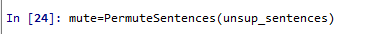
\includegraphics[width=0.7\textwidth]
      {figures/cokro/c100}}
      \caption{Membuat variabel mute}
      \label{c100}
      \end{figure}

\begin{figure}[!htbp]
      \centering{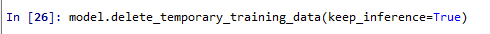
\includegraphics[width=0.7\textwidth]
      {figures/cokro/c101}}
      \caption{Code Pembersihan}
      \label{c101}
      \end{figure}

\item kenapa model harus di save ? suapaya dalam pengolahan data tidak perlu menjalankan kembali data vektorisasi serta untuk meringankan beban ram. kemudian temporary harus dihapus guna meningkatkan peforma komputer. adapun codenya dapat dilihat pada gambar \ref{c102} dan untuk hasil simpan datanya dapat di lihat pada gambar \ref{c103}.

\begin{figure}[!htbp]
      \centering{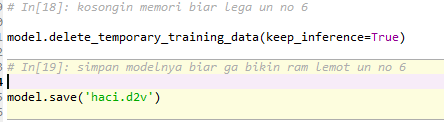
\includegraphics[width=0.7\textwidth]
      {figures/cokro/c102}}
      \caption{Membuat variabel mute}
      \label{c102}
      \end{figure}

\begin{figure}[!htbp]
      \centering{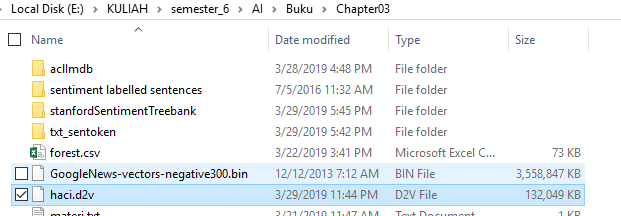
\includegraphics[width=0.7\textwidth]
      {figures/cokro/c103}}
      \caption{Hasil save data vektorisasi}
      \label{c103}
      \end{figure}

\item inver\_code digunakan untuk membandingkan data doc2vec yang telah di olah dengan kata yang baru atau data yang ada dalam perintah vector itu sendiri contoh membandingkan kata (i will go home) untuk lebih jelasnya dapat di lihat pada gambar \ref{c104}. kemudian untuk hasil running code tersebut dapat di lihat pada gambar \ref{c105} pada hasil gambar tersebut terdapat hasil vektor yang rata rata berada pada kisaran 0,2 an yang berarti kata yang dimasukan pada inter\_vec datanya ada pada doc2vec atau ada data yang bobotnya menyamai kata-kata di dalam dokumen tersebut.

\begin{figure}[!htbp]
      \centering{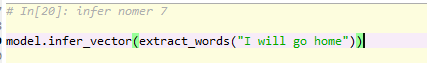
\includegraphics[width=0.7\textwidth]
      {figures/cokro/c104}}
      \caption{Code untuk inver\_code}
      \label{c104}
      \end{figure}

\begin{figure}[!htbp]
      \centering{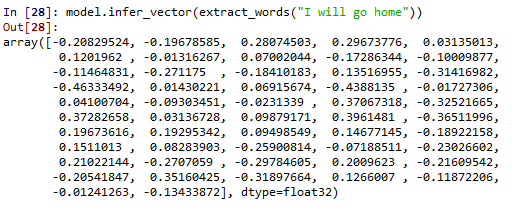
\includegraphics[width=0.7\textwidth]
      {figures/cokro/c105}}
      \caption{Hasil dari inver code}
      \label{c105}
      \end{figure}

\item consine\_simirarity setelah melakukan pengolahan data doc2vec dilakukan consine simirarity yang bertujuan untuk membandingkan data berisikan bahasa inggris dengan data yang telah di olah tadi apakah hasilnya mirip atau tidak untuk caranya yaitu dengan cara mencobacodingan yang terdapat pada gambar \ref{c106} berikut maka akan muncul hasilnya berapa persen dengan tulisan 0.4 sekian yang berarti tingkat kemiripan dokumen yang di uji tadi untuk hasilnya dapat dilihat pada gambar \ref{c107} berikut.

\begin{figure}[!htbp]
      \centering{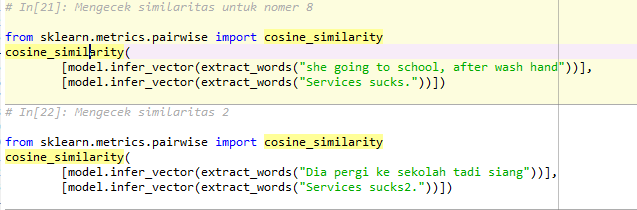
\includegraphics[width=0.7\textwidth]
      {figures/cokro/c106}}
      \caption{Code untuk consine\_simirarity}
      \label{c106}
      \end{figure}

\begin{figure}[!htbp]
      \centering{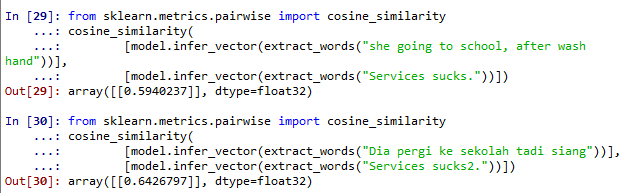
\includegraphics[width=0.7\textwidth]
      {figures/cokro/c107}}
      \caption{Hasil dariconsine\_simirarity}
      \label{c107}
      \end{figure}

\item untuk melakukan cross validation pertama masukan terlebih dahulu metode KNeighborsClasifier dan RandomForestClasifier dari library sklearn kemudian dilakukan cross validation setelah itu buat variabel clf dengan isi KNeighborsClasifier dan variabel clfrf dengan isi RandomForestClasifier kemudian di buat skor menggunakan cross validation dengan menggunakan variabel clf dan data sentvecs dan sentiments kemudian dengan numpy dibuat mean dari scores begitu pula untuk variabel clfrf selanjutnya melakukan import metode make\_pipeline yang dilakukan untuk membuat skor dari vektorisasi tfidf dan rf. untuk lebih jelasnya dapat di lihat pada gambar \ref{c108}  maka akan muncul hasil rata-rata 0,76 sekian atau 76 persen untuk clf yang dapat dilihat pada gambar \ref{c109} dan untuk hasil clfrf menghasilkan hasil rata-rata di 71 persen yang dapat dilihat pada gambar \ref{c110} dan untuk hasil rata-rata keseluruhan cros validation sebesar 0,74 atau 74 persen yang dapat dilihat pada gambar \ref{c109}.

\begin{figure}[!htbp]
      \centering{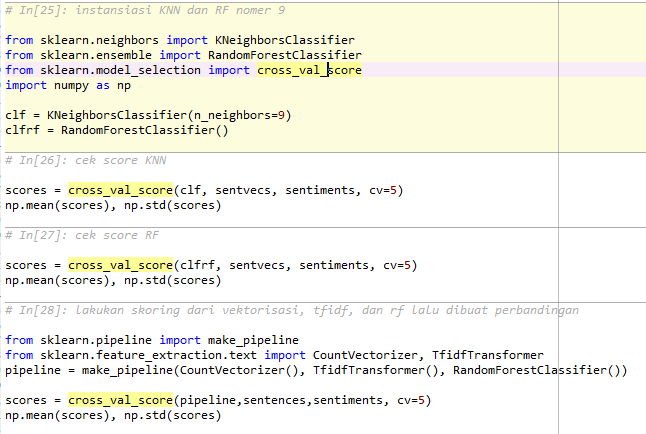
\includegraphics[width=0.7\textwidth]
      {figures/cokro/c108}}
      \caption{Code untuk Cros Validation}
      \label{c108}
      \end{figure}

\begin{figure}[!htbp]
      \centering{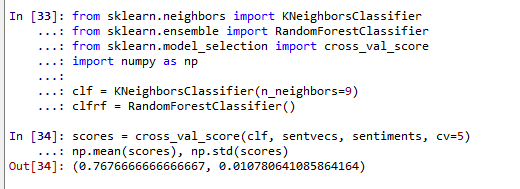
\includegraphics[width=0.7\textwidth]
      {figures/cokro/c109}}
      \caption{Hasil dari perhitungan KNeighborsClasifier}
      \label{c109}
      \end{figure}

\begin{figure}[!htbp]
      \centering{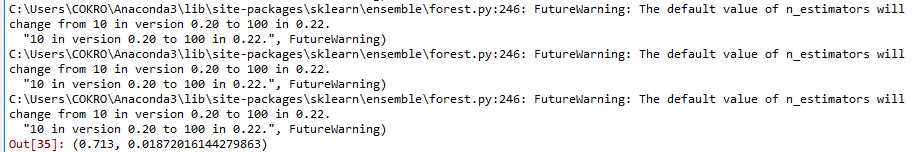
\includegraphics[width=0.7\textwidth]
      {figures/cokro/c110}}
      \caption{Hasil dari perhitungan RandomForestClasifier}
      \label{c110}
      \end{figure}

\begin{figure}[!htbp]
      \centering{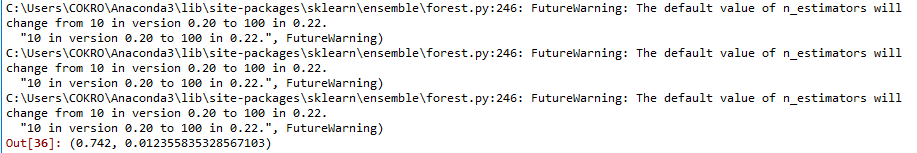
\includegraphics[width=0.7\textwidth]
      {figures/cokro/c111}}
      \caption{Hasil dari perhitungan Cross Validation 1}
      \label{c111}
      \end{figure}

\begin{figure}[!htbp]
      \centering{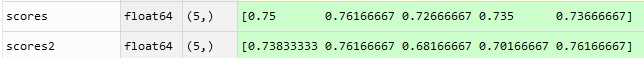
\includegraphics[width=0.7\textwidth]
      {figures/cokro/c112}}
      \caption{Hasil dari perhitungan Cross Validation 2}
      \label{c112}
      \end{figure}

\end{enumerate}
\subsection{Penanganan Error}



\section{Fathi Rabbani / 1164074}
\subsection{Teori}
\begin{enumerate}
\item Why words need to be Vectorizer
\subitem karena kata - kata yang digunakan untuk memproses data agar dapat menjadi bagian dati kumpulan data atatu atribut yang dapat dibaca oleh sistem machine learning karena sistem tersebut tidak dapat memproses data text secara langsung dan harus di convert terlebih dahulu kedalam bilangan.untuk ilustrasinya dapat dilihat pada gambar \ref{fig1}
\begin{figure}[!htbp]
	\centering
	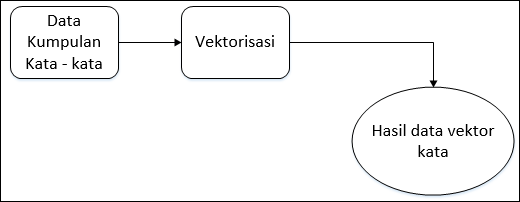
\includegraphics[width=0.5\textwidth]{figures/fathi/chapter5/hari1/1}
	\caption{Ilustrasi Vektorisasi Kata}
	\label{fig1}
\end{figure}

\item Why Dimension of Google dataset can reach 300
\subitem Dimensi dataset dari google bisa mencapai 300 karena dimensi dari vektor tersebut digunakan untuk membandingkan bobot dari setiap data kata yang diproses. ilustrasi dapat dilihat pada gambar \ref{fig2}
\begin{figure}[!htbp]
	\centering
	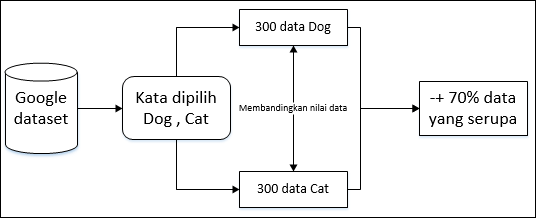
\includegraphics[width=0.5\textwidth]{figures/fathi/chapter5/hari1/2}
	\caption{Ilustrasi Google dataset}
	\label{fig2}
\end{figure}

\item Concept of Vectorizer on words
\subitem pada vektorisasi dengan menggunakan Word2Vec memiliki kelebihan yang dapat dibedakan dengan pengguaan bag of words yang biasanya.  pada bag of word pemrosesan data tidak dapat menganalisa data yang memiliki makna sama namun penulisannya berbeda, namun pada penggunaan Word2Vec proses tersebut dapat berjalan dengan lebih mudah contohnya adalah penulisan kata please dengan plz. untuk ilustrasi datanya bisa dilihat dalam gambar \ref{fig3}
\begin{figure}[!htbp]
	\centering
	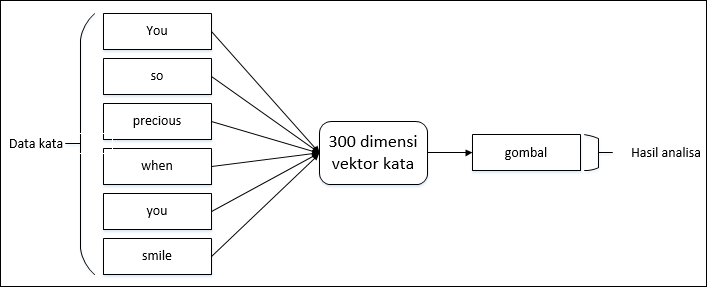
\includegraphics[width=0.5\textwidth]{figures/fathi/chapter5/hari1/3}
	\caption{Ilustrasi Concept of Vectorizer on Words}
	\label{fig3}
\end{figure}

\item Concept of Vectorizer on documents
\subitem vektorisasi pada Doct2Vec dimana data yang terdapat pada file document tersebut diolah dengan melakukan pemrosesan yang mengutamakan nilai data filenamenya atau atribut utama dimana nilai data inputnya tidak terlalu diproses. ilustrasinya dapat dilihat pada gambar \ref{fig4}
\begin{figure}[!htbp]
	\centering
	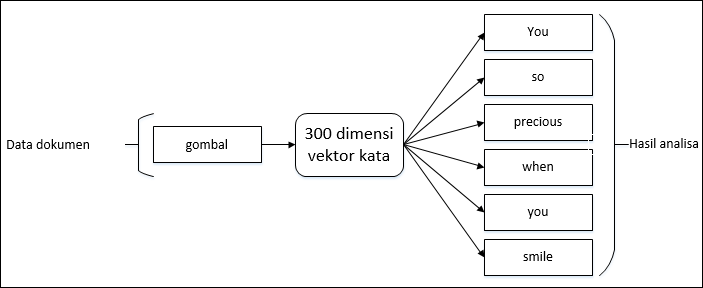
\includegraphics[width=0.5\textwidth]{figures/fathi/chapter5/hari1/4}
	\caption{Ilustrasi Concept of Vectorizer on Document}
	\label{fig4}
\end{figure}

\item What is mean and deviation standart
\subitem Mean adalah nilai rata-rata dari beberapa buah data. Nilai mean dapat ditentukan dengan membagi jumlah data dengan banyaknya data.

\subitem Standar deviasi adalah nilai statistik yang digunakan untuk menentukan bagaimana sebaran data dalam sampel, dan seberapa dekat titik data individu ke mean – atau rata-rata – nilai sampel.

untuk ilustrasi data mean dan deviation standart bisa dilihat pada gambar \ref{fig5}
\begin{figure}[!htbp]
	\centering
	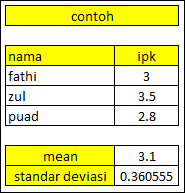
\includegraphics[width=0.5\textwidth]{figures/fathi/chapter5/hari1/5}
	\caption{Ilustrasi Mean and Deviation Standart}
	\label{fig5}
\end{figure}

\item What is skip-gram
\subitem Skip-gram merupakan teknik yang digunakan di area speech processing, dimana n-gram yang dibentuk kemudian ditambahkan juga dengan tindakan “skip” pada token-tokennya. contohnya terdapat pada gambar \ref{fig6}
\begin{figure}[!htbp]
	\centering
	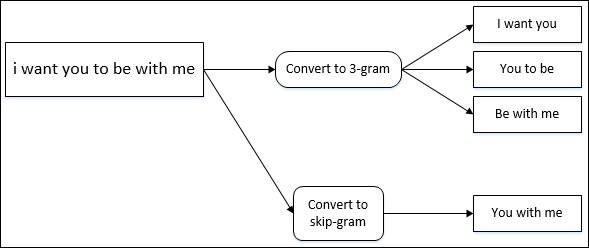
\includegraphics[width=0.5\textwidth]{figures/fathi/chapter5/hari1/6}
	\caption{Ilustrasi  skip-gram}
	\label{fig6}
\end{figure}
\end{enumerate}

\subsection{Praktikum}
\begin{enumerate}
\item Try datasets GoogleNews-vectors
\begin{itemize}
\item berikut adalah hasil dari code yang digunakan untuk memanggil data library GENSIM dengan menggunakan perintah import, lalu dari library tersebut diambillah data yang akan digunakan untuk memproses data dari GoogleNews-vector. ilustrasi dapat dilihat pada gambar \ref{fig7}
\begin{figure}[!htbp]
	\centering
	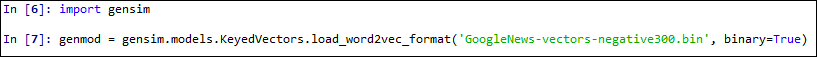
\includegraphics[width=0.8\textwidth]{figures/fathi/chapter5/hari2/1}
	\caption{Ilustrasi  import gensim dan olah data GoogleNews-vector}
	\label{fig7}
\end{figure}

\item lalu pada penggunaan code berikut ini akan mengolah data LOVE yang terdapat pada file GoogleNews-vector, hasil dari pemrosesannya dapat dilihat pada gambar \ref{fig8}
\begin{figure}[!htbp]
	\centering
	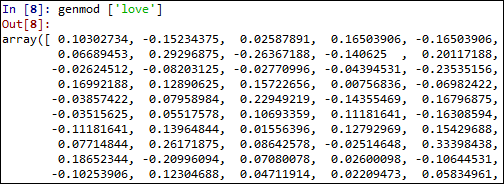
\includegraphics[width=0.5\textwidth]{figures/fathi/chapter5/hari2/2}
	\caption{Ilustrasi hasil olah data LOVE pada GoogleNews-vector}
	\label{fig8}
\end{figure}

\item  lalu pada penggunaan code berikut ini akan mengolah data FAITH yang terdapat pada file GoogleNews-vector, hasil dari pemrosesannya dapat dilihat pada gambar \ref{fig8}
\begin{figure}[!htbp]
	\centering
	\includegraphics[width=0.5\textwidth]{figures/fathi/chapter5/hari2/3}
	\caption{Ilustrasi hasil olah data FAITH pada GoogleNews-vector}
	\label{fig8}
\end{figure}

\item  lalu pada penggunaan code berikut ini akan mengolah data FALL yang terdapat pada file GoogleNews-vector, hasil dari pemrosesannya dapat dilihat pada gambar \ref{fig9}
\begin{figure}[!htbp]
	\centering
	\includegraphics[width=0.5\textwidth]{figures/fathi/chapter5/hari2/4}
	\caption{Ilustrasi hasil olah data FALL pada GoogleNews-vector}
	\label{fig9}
\end{figure}

\item  lalu pada penggunaan code berikut ini akan mengolah data SICK yang terdapat pada file GoogleNews-vector, hasil dari pemrosesannya dapat dilihat pada gambar \ref{fig10}
\begin{figure}[!htbp]
	\centering
	\includegraphics[width=0.5\textwidth]{figures/fathi/chapter5/hari2/5}
	\caption{Ilustrasi hasil olah data SICK pada GoogleNews-vector}
	\label{fig10}
\end{figure}

\item  lalu pada penggunaan code berikut ini akan mengolah data CLEAR yang terdapat pada file GoogleNews-vector, hasil dari pemrosesannya dapat dilihat pada gambar \ref{fig11}
\begin{figure}[!htbp]
	\centering
	\includegraphics[width=0.5\textwidth]{figures/fathi/chapter5/hari2/6}
	\caption{Ilustrasi hasil olah data CLEAR pada GoogleNews-vector}
	\label{fig11}
\end{figure}

\item  lalu pada penggunaan code berikut ini akan mengolah data SHINE yang terdapat pada file GoogleNews-vector, hasil dari pemrosesannya dapat dilihat pada gambar \ref{fig12}
\begin{figure}[!htbp]
	\centering
	\includegraphics[width=0.5\textwidth]{figures/fathi/chapter5/hari2/7}
	\caption{Ilustrasi hasil olah data SHINE pada GoogleNews-vector}
	\label{fig12}
\end{figure}

\item  lalu pada penggunaan code berikut ini akan mengolah data BAG yang terdapat pada file GoogleNews-vector, hasil dari pemrosesannya dapat dilihat pada gambar \ref{fig13}
\begin{figure}[!htbp]
	\centering
	\includegraphics[width=0.5\textwidth]{figures/fathi/chapter5/hari2/8}
	\caption{Ilustrasi hasil olah data BAG pada GoogleNews-vector}
	\label{fig13}
\end{figure}

\item  lalu pada penggunaan code berikut ini akan mengolah data CAR yang terdapat pada file GoogleNews-vector, hasil dari pemrosesannya dapat dilihat pada gambar \ref{fig14}
\begin{figure}[!htbp]
	\centering
	\includegraphics[width=0.5\textwidth]{figures/fathi/chapter5/hari2/9}
	\caption{Ilustrasi hasil olah data CAR pada GoogleNews-vector}
	\label{fig14}
\end{figure}

\item  lalu pada penggunaan code berikut ini akan mengolah data WASH yang terdapat pada file GoogleNews-vector, hasil dari pemrosesannya dapat dilihat pada gambar \ref{fig15}
\begin{figure}[!htbp]
	\centering
	\includegraphics[width=0.5\textwidth]{figures/fathi/chapter5/hari2/10}
	\caption{Ilustrasi hasil olah data WASH pada GoogleNews-vector}
	\label{fig15}
\end{figure}

\item  lalu pada penggunaan code berikut ini akan mengolah data MOTOR yang terdapat pada file GoogleNews-vector, hasil dari pemrosesannya dapat dilihat pada gambar \ref{fig16}
\begin{figure}[!htbp]
	\centering
	\includegraphics[width=0.5\textwidth]{figures/fathi/chapter5/hari2/11}
	\caption{Ilustrasi hasil olah data MOTOR pada GoogleNews-vector}
	\label{fig16}
\end{figure}

\item  lalu pada penggunaan code berikut ini akan mengolah data CYCLE yang terdapat pada file GoogleNews-vector, hasil dari pemrosesannya dapat dilihat pada gambar \ref{fig17}
\begin{figure}[!htbp]
	\centering
	\includegraphics[width=0.5\textwidth]{figures/fathi/chapter5/hari2/12}
	\caption{Ilustrasi hasil olah data CYCLE pada GoogleNews-vector}
	\label{fig17}
\end{figure}

\item  dan pada hasil code berikut ini adalah hasil dari proses penggunaan perintah code similarity yang akan menghitung nilai value data yang dibandingkan dengan masing - masing kata seperti pada hasil dari perbandingan kata LOVE disandingkan dengan FAITH menghasilkan nilai 37 persen, sedangkan kata WASH dan SHINE menghasilkan nilai 27 persen dan kata CAR yang disandingkan dengan kata MOTOR menghasilkan 48 persen, dimana kita dapat menyimpulkan bahwa semakin data kata tersebut memiliki tingkat kesamaan yang tinggi maka nilai hasil yang ditampilkanpun akan semakin tinggi. ilustrasi bisa dilihat pada gambar \ref{fig18}
\begin{figure}[!htbp]
	\centering
	\includegraphics[width=0.5\textwidth]{figures/fathi/chapter5/hari2/13}
	\caption{Ilustrasi hasil olah data  pada GoogleNews-vector menggunakan SIMILARITY}
	\label{fig18}
\end{figure}
\end{itemize}

\item extract\_words dan PermutedSentences
\subitem pada penjelasan berikut ini akan menyangkut pembersihan data yang akan digunakan untuk diproses, dimana data akan di EXTRACT dari setiap katanya agar terbebas dari data TAG HTML, APOSTROPHES, TANDA BACA, dan SPASI yang berlebih. dengan menggunakan perintah code STRIP dan SPLIT. lalu penggunaan library random yang akan dibuat untuk melakukan KOCLOK data dengan acuan datanya adalah data yang terdapat pada variable KATA. untuk ilustrasi hasil dari codenya dapat dilihat pada gambar \ref{fig19}
\begin{figure}[!htbp]
	\centering
	\includegraphics[width=0.5\textwidth]{figures/fathi/chapter5/hari2/14}
	\caption{Ilustrasi hasil olah data  pada GoogleNews-vector menggunakan extract\_words dan PermuteSentences}
	\label{fig19}
\end{figure}

\item TaggedDocument dan Doc2Vec
\subitem gensim merupakan open-source model ruang vektor dan toolkit topic modeling, yang diimplementasikan dalam bahasa pemrograman Python. Untuk kinerja Gensim, digunakan NumPy, SciPy dan Cython (opsional). Gensim secara khusus ditujukan untuk menangani koleksi teks besar dengan menggunakan algoritma secara online. Gensim mengimplementasikan tf-idf, latent semantic analysis (LSA), Latent Dirichlet Analysis (LDA), dan lain-lain. 
\subitem tagged document merupakan sebuah class yang terdapat pada pemrosesan data pada library gensim yang akan mengolah data teks yang ada pada dokumen - dokumen yang dipakai.
\subitem Doc2Vec merupakan algoritma doct embedding, yaitu pemetaan dari dokumen menjadi vektor, serta pemetaan data dokumen 1 dan dokumen lainnya.
ilustrasi dari tagged document dan Word2Vec ada pada gambar \ref{fig20}
\begin{figure}[!htbp]
	\centering
	\includegraphics[width=0.5\textwidth]{figures/fathi/chapter5/hari3/1}
	\caption{Ilustrasi TaggedDocument dan Doc2Vec }
	\label{fig20}
\end{figure}

\item Praktek data training
\subitem pertama buka data training yang akan diolah pada aplikasi python, import library OS dan membuat data variable unsup\_senteces dengan nilai array kosong. buatkan data direktori untuk memanggil data yang akan diolah dan buatkan juga variable data nilai fname yang akan memproses data dirname untuk diisikan pada variable unsup\_sentences. code yang digunakan dapat dilihat pada gambar \ref{fig21}
\begin{figure}[!htbp]
	\centering
	\includegraphics[width=0.5\textwidth]{figures/fathi/chapter5/hari3/2}
	\caption{Ilustrasi data code praktek data training }
	\label{fig21}
\end{figure}

data pada hasil code digambar berikut \ref{fig22}, menghasilkan data pada gambar \ref{fig23} yang akan memunculkan data variable DIRNAME, FNAME, KATA dan unsup\_sentences yang memiliki data sebanyak 55 kata dalam file yang diolah tersebut. hasil run dengan menggunakan code pada gambar \ref{fig24}, menghasilkan data nilai yang terdapat pada gambar \ref{fig25}. lalu pada code yang terdapat digambar \ref{fig26}, menghasilkan data \ref{fig27}.
\begin{figure}[!htbp]
	\centering
	\includegraphics[width=0.5\textwidth]{figures/fathi/chapter5/hari3/3}
	\caption{Ilustrasi data code praktek data training }
	\label{fig22}
\end{figure}
\begin{figure}[!htbp]
	\centering
	\includegraphics[width=0.5\textwidth]{figures/fathi/chapter5/hari3/4}
	\caption{Ilustrasi data code praktek data training }
	\label{fig23}
\end{figure}
\begin{figure}[!htbp]
	\centering
	\includegraphics[width=0.5\textwidth]{figures/fathi/chapter5/hari3/5}
	\caption{Ilustrasi data code praktek data training }
	\label{fig24}
\end{figure}
\begin{figure}[!htbp]
	\centering
	\includegraphics[width=0.5\textwidth]{figures/fathi/chapter5/hari3/6}
	\caption{Ilustrasi data code praktek data training }
	\label{fig25}
\end{figure}
\begin{figure}[!htbp]
	\centering
	\includegraphics[width=0.5\textwidth]{figures/fathi/chapter5/hari3/7}
	\caption{Ilustrasi data code praktek data training }
	\label{fig26}
\end{figure}
\begin{figure}[!htbp]
	\centering
	\includegraphics[width=0.5\textwidth]{figures/fathi/chapter5/hari3/8}
	\caption{Ilustrasi data code praktek data training }
	\label{fig27}
\end{figure}

\item Why need Shuffled and Clean memory
\subitem dilakukan shuffled adalah agar datanya lebih mudah untuk diolah dan untuk menentukan tingkat tinggi akurasi dari hasil pemrosesan. dan dilakukan pembersihan memory adalah agar chace yang disimpan tidak membuat proses pada komputer mejadi lambat dan dapat digunakan untuk memproses data lainnya agar menjadi lebih ringan dan cepat.
pada gambar \ref{fig28} adlah proses untuk melakukan pengoclokan data dan pada gambar \ref{fig29} adalah proses untuk memasukan data unsup\_sentences kedalam variable muter untuk diproses dengan class PermuterSentences. dan pada gambar \ref{30} adalah code yang digunakan untuk membersihkan data memory.
\begin{figure}[!htbp]
	\centering
	\includegraphics[width=0.5\textwidth]{figures/fathi/chapter5/hari3/9}
	\caption{Ilustrasi Shuffled dan Randomisasi data }
	\label{fig28}
\end{figure}
\begin{figure}[!htbp]
	\centering
	\includegraphics[width=0.5\textwidth]{figures/fathi/chapter5/hari3/10}
	\caption{Ilustrasi pembuatan variable muter untuk memuat data unsup\_sentences}
	\label{fig29}
\end{figure}
\begin{figure}[!htbp]
	\centering
	\includegraphics[width=0.5\textwidth]{figures/fathi/chapter5/hari3/11}
	\caption{Ilustrasi code untuk membersihkan data memory}
	\label{fig30}
\end{figure}


\item Why model have to be saved
\subitem dalam pengolahan data dengan menggunakan proses yang panjang ditakutkan data yang sudah diproses tersebut dapat hilang jika terdapat kejadian atau emergency pada saat pengolahan dan pemrosesan data, misalnya harddisk error atau pun listrik yang padam. dan proses penyimpanan data juga dilakukan agar data yang sudah diolah data dipanggil lagi tanpa harus melakukan proses dari awal sehingga tidak memakan waktu. untuk code yang digunakan dapat dilihat pada gambar \ref{fig31}

\begin{figure}[!htbp]
	\centering
	\includegraphics[width=0.5\textwidth]{figures/fathi/chapter5/hari3/12}
	\caption{Ilustrasi data code save data}
	\label{fig31}
\end{figure}

berikut ini adalah hasil file dari penggunaan code save tersebut. bisa dilihat pada gambar \ref{fig32}
\begin{figure}[!htbp]
	\centering
	\includegraphics[width=0.5\textwidth]{figures/fathi/chapter5/hari3/13}
	\caption{Ilustrasi hasil file simpan}
	\label{fig32}
\end{figure}

\item infer\_vector
\subitem berfungsi untuk dokumen baru, dan  bisa menggunakan data vektor yang dilatih secara massal, seperti yang disimpan dalam model, untuk dokumen yang merupakan bagian dari data training. untuk percobaannya dapat dilihat pada gambar \ref{33}
\begin{figure}[!htbp]
	\centering
	\includegraphics[width=0.5\textwidth]{figures/fathi/chapter5/hari3/14}
	\caption{Ilustrasi code dan hasil infer\_vector}
	\label{fig33}
\end{figure}

\item cosine\_similarity
\subitem merupakan sebuah algoritma yang digunakan untuk membandingkan dari dua buah data yang bukan merupakan data vector untuk menguji nilai kemiripan data satu dengan data lainnya. hasil dari percobaan pada tugas no 8 ini dapat dilihat pada gambar \ref{fig34} yang menghasilkan nilai akurasi sebesar 20 persen dan gambar \ref{fig35} yang menghasilkan nilai akurasi sebesar 91 persen.
\begin{figure}[!htbp]
	\centering
	\includegraphics[width=0.5\textwidth]{figures/fathi/chapter5/hari4/1}
	\caption{Ilustrasi code dan hasil penggunaan cosine\_similarity}
	\label{fig34}
\end{figure}

\begin{figure}[!htbp]
	\centering
	\includegraphics[width=0.5\textwidth]{figures/fathi/chapter5/hari4/2}
	\caption{Ilustrasi code dan hasil penggunaan cosine\_similarity}
	\label{fig35}
\end{figure}

\item Cross Validation
\subitem pertama melakukan import data dari library KNeighborsClassifier, RandomForestClassifier, cross\_val\_score dan numpy yang digunakan untuk membuat data cross validasi dapat dilihat pada gambar \ref{fig36}.
\begin{figure}[!htbp]
	\centering
	\includegraphics[width=0.5\textwidth]{figures/fathi/chapter5/hari4/3}
	\caption{Ilustrasi memasukan code import library}
	\label{fig36}
\end{figure}

\subitem lalu selanjutnya membuat data variable scores yang akan memuat nilai cross\_val\_score dengan datanya diambil dari KNeighborsClassifier yang terdiri dari sentvecs, sentiments dan clf dan mengolahnya menggunakan numpy untuk menampilkan data pada gambar \ref{fig37}yang menghasilkan nilai akurasi sebesar 53 persen.
\begin{figure}[!htbp]
	\centering
	\includegraphics[width=0.5\textwidth]{figures/fathi/chapter5/hari4/4}
	\caption{Ilustrasi perhitungan data KNeighborsClassifier dengan cross validasi}
	\label{fig37}
\end{figure}

\subitem membuat data variable scores yang akan memuat nilai cross\_val\_score dengan datanya diambil dari RandomForestClassifier yang terdiri dari sentvecs, sentiments dan clfrf dan mengolahnya menggunakan numpy untuk menampilkan data pada gambar \ref{fig38} yang menghasilkan nilai akurasi sebesar 53 persen. 
\begin{figure}[!htbp]
	\centering
	\includegraphics[width=0.5\textwidth]{figures/fathi/chapter5/hari4/5}
	\caption{Ilustrasi perhitungan data  RandomForestClassifier dengan cross validasi}
	\label{fig38}
\end{figure}

\subitem penggunaan make\_pipeline adalah untuk membuat data dari KNeighborsClassifier, RandomForestClassifier dan Vectorizer digabungkan untuk menghasilkan data nilai pada gambar\ref{fig39} menghasilkan nilai akurasi sebesar 74 persen. 
\begin{figure}[!htbp]
	\centering
	\includegraphics[width=0.5\textwidth]{figures/fathi/chapter5/hari4/6}
	\caption{Ilustrasi perhitungan data Cross Validasi untuk nilai keseluruhan dari KNeighborsClassifier, RandomForestClassifier dan Vectorizer}
	\label{fig39}
\end{figure}

dan keseluruhan nilai yang tercatat terdapat pada gambar \ref{fig40}.
\begin{figure}[!htbp]
	\centering
	\includegraphics[width=0.5\textwidth]{figures/fathi/chapter5/hari4/7}
	\caption{Ilustrasi perhitungan data hasil persenan yang diakumulasi}
	\label{fig40}
\end{figure}

\end{enumerate}